%!TEX root = book.tex 
% springer volume on vagueness & rationality
%%%%%%%%%%%%%%%%%%%%% chapter.tex %%%%%%%%%%%%%%%%%%%%%%%%%%%%%%%%%
%
% sample chapter
%
% Use this file as a template for your own input.
%
%%%%%%%%%%%%%%%%%%%%%%%% Springer-Verlag %%%%%%%%%%%%%%%%%%%%%%%%%%
\motto{This is a \textsf{motto}:  Use the template \emph{chapter.tex} to style the various elements of your chapter content.}
%% \bibliographystyle{spbasic}
%% spbasic info
% This is an author-year citation style bibliography. As such, it is non-standard LaTeX, and requires a special package file to function properly. Such a package is natbib.sty by Patrick W. Daly
% For Springer medical, life sciences, chemistry, geology, engineering and computer science publications.   
% For use with the natbib package (see below). Default is author-year citations. When citations are numbered, please use \usepackage[numbers]{natbib}.
% The \cite command functions as follows:
 %   \citet{key} ==>>                Jones et al. (1990)
 %   \citet*{key} ==>>               Jones, Baker, and Smith (1990)
 %   \citep{key} ==>>                (Jones et al., 1990)
 %   \citep*{key} ==>>               (Jones, Baker, and Smith, 1990)
 %   \citep[chap. 2]{key} ==>>       (Jones et al., 1990, chap. 2)
 %   \citep[e.g.][]{key} ==>>        (e.g. Jones et al., 1990)
 %   \citep[e.g.][p. 32]{key} ==>>   (e.g. Jones et al., p. 32)
 %   \citeauthor{key} ==>>           Jones et al.
 %   \citeauthor*{key} ==>>          Jones, Baker, and Smith
 %   \citeyear{key} ==>>             1990
\chapter{The Elusive Benefits of Vagueness: the Evidence So Far}
\label{intro} % Always give a unique label
% use \chaptermark{}
% to alter or adjust the chapter heading in the running head



\abstract{Much of everyday language is vague, yet the benefits of vagueness for hearers and readers are proving to be elusive. We discuss a range of earlier controlled experiments with human participants, and we report on a new series of experiments that we conducted in recent years. These new experiments, which focus on vague expressions that are part of referential noun phrases, aim to separate the utility of vagueness (as defined by the existence of borderline cases, as is common in theoretical work on vagueness) from the utility of other factors that tend to co-occur with vagueness. Having presented the evidence, we argue that the evidence so far supports a view of vagueness where the benefits that vague terms exert are due to other influences, rather than to vagueness itself. These factors include: low granularity; the use of evaluative words; the avoidance of overtly numerical words; the existence of comparison strategies; and, lastly and more tentatively, a phenomenon that we call range reduction. Although it is possible that other types of vague expressions (i.e., vague words outside referential noun phrases) behave differently, our work suggests that vagueness itself may not increase the utility of an expression.}

\section{Introduction}
\label{sec:1}

Vagueness pervades the language that we use on a daily basis. In everyday use, language use may be called vague for various reasons -- see e.g. the entry for \emph{vague} in \cite{penguin}.  In most academic use though, the word \emph{vagueness} has a more particular meaning. \citeauthor{keefe1997vagueness}, for example, state \begin{quotation}vague predicates have borderline cases, have fuzzy boundaries, and are susceptible to sorites paradoxes \cite[p.\ 4]{keefe1997vagueness}\end{quotation} (a similar definition can be found in \cite{EgreKlinedinst}, among many others).  The most crucial of these criteria is the existence of borderline cases: \begin{quotation}a word is precise if it describes a well-defined set of objects. By contrast, a word is vague if it is not precise \cite[p.\ 1]{lipmanvague}\end{quotation} A typical example is the word \emph{tall}, as applied to people for example, because here is no precise, known height which separates those who are tall from those who are not. The crucial point is that \emph{tall} admits borderline cases (i.e., people who may or may not count as tall), which are the hallmark of vagueness as we use the term.

Linguists, philosophers of language, and more recently game theorists, have asked why natural languages contain so many vague expressions, which are used so frequently \cite{Lipman:2000fk, lipmanvague}. By introducing borderline cases, these expressions create potential misunderstandings, thereby creating \begin{quotation}a worldwide several-thousand year efficiency loss \cite[p.\ 1]{lipmanvague}\end{quotation} \citeauthor{lipmanvague} explains the point by means of a scenario in which a speaker describes a person to a hearer, who needs to identify that person in the arrivals hall of of an airport. Lipman argues that, in such a scenario, a precise description of the person's height, e.g., \textsl{The person's height is 187.96~cm} would be more useful than a vague one, e.g., \textsl{The person is tall}. Lipman uses this scenario to explain why standard game theory models of communication, \citep[e.g.][]{Crawford:1982lr} predict that, under certain conditions, a crisp act of communication will always have more utility than a vague act that communicates the same state of affairs. The relevant conditions are, broadly speaking, that both interlocutors know all the relevant facts (e.g., both know the person's height precisely) and that the setting for the communication is co-operative. These conditions exclude deliberate deception, and rhetorical situations like political debate and advertising where the intention is to persuade the interlocutor to adopt some point of view, where the persuasion might not be intended to be in the addressee's best interest. 

Lipman argued that such the efficiency loss resulting from vague expressions would be unlikely to have arisen unless there are advantages as well as disadvantages associated with vague expressions. Lipman asked, essentially, what these advantages might be, and how they might find a place in a game-theoretical explanation. In this paper, we focus on the first part of Lipman's question.

Several tentative answers to Lipman's question have been offered -- see \citet{van2009utility, van2010vagueness}. Prominent among these answers is the idea that vague expressions are somehow easier to process, by a speaker and/or a hearer, than expressions that are not \emph{vague}, i.e., that are \emph{crisp} \citep[e.g.,][]{lipmanvague,De-Jaegher:2003lr,vanrooij2003lr}. For example, Lipman writes: \begin{quotation}For the listener, information which is too specific may require more effort to analyze \citep[][p.\ 11]{lipmanvague}  \end{quotation} We shall refer to this characterisation of the utility of vague language as the \emph{cost reduction} hypothesis. The idea of vagueness as cost reduction can take various shapes, but the basic hypothesis is that it is easier for people to think in terms of loosely defined categories, such as \emph{quite a few}, or \emph{many}, than in terms of crisply defined ones, such as \emph{thirteen}, or \emph{237}. This predicts that whenever a vague expression can perform the same communicative task as a crisp one, it is rational to choose the vague expression. The corollary for comprehension is that vague expressions should be understood more readily than precise expressions. 

Questions concerning optimal language use have many practical applications. Natural Language Generation\footnote{\textsc{nlg} systems take data or formulas as input, and transform them into natural language outputs \cite[][]{reiter2000building}. The process parallels language production in humans.}  (henceforth \textsc{nlg}) systems must make decisions between different formulations of the same information. For example, if a man's height is 6 foot 2 inches, this could be expressed as \emph{187.96 metres}, \emph{6 foot 2}, or \emph{tall}, among other ways, and the \textsc{nlg} system must decide between these.  The problem is particularly relevant for \textsc{nlg} systems that take numbers as input, as many do. In the context of an \textsc{nlg} system faced with a practical decision of this kind, Lipman's question becomes \emph{Under what circumstances should vague terms be produced?}  Relevant applications include weather forecasting on the basis of numerical weather data such as temperature and wind speed \citep{goldberg1994using, turner2006generating}, and medical decision support on the basis of clinical measurement such as oxygen saturation, heart rhythm, etc. \citep{Hripcsak01032009, hunter2008summarising, portet2009automatic}. At present, such \textsc{nlg} systems are often forced to make decisions concerning the level of precision in the utterances that they generate (e.g., \emph{the temperature will be in the high twenties tomorrow}) on the basis of little more than intuition. A better understanding of the benefits of different precision levels for readers would allow these systems to become more useful. 

The cost reduction hypothesis is of direct relevance to psycholinguists interested in language comprehension, and additionally to psycholinguists interested in language production, for example in connection with the question of audience design \citep{Clark1982287}. For, to the extent that speakers and writers choose vague expressions over and above crisp ones because the former are easier to process for hearers than the latter, the cost reduction hypothesis suggests that speakers design their utterance for optimal benefit to their hearers -- out of altruism, so to speak.

The utility of vagueness is the attested aim of a small number of studies, but most of these have focussed on vagueness in a different sense, and focussing on different types of benefits for hearers. Two recent studies can illustrate both issues. 

\paragraph{Behaviour modification experiments} 
In a series of studies of behaviour modification, \citet[]{Mishra01042011} manipulated the presentation format of information about quantities in the domains of mental acuity, physical strength, and weight loss. In the weight loss study, participants were told that the study was designed to test the validity of a new (actually fictitious) health index, the HHI (Holistic Health Index). They were told that an ideal HHI score lies in the range of 45 to 55. In a longitudinal study, participants submitted their height, weight, hydration level, gender, and age to a computer each week. Participants were told that two algorithms would be used to compute their HHI, and that it was possible that the two algorithms might give different values initially, but would converge over the course of the study to a single value. They were also told that if the two algorithms did give different values, then the true score lay between the two values. In one condition, which the authors called the precise condition, the two algorithms gave the same score. In the other condition, which the authors called the vague condition, one algorithm added 3\% to the score while the other algorithm subtracted 3\% from the score, yielding a range of values whose midpoint was the same as the two values given in the precise condition. 

\paragraph{Ratings experiments} 
Similar issues arise from the work of \citet{peters2009bringing}. The authors carried out a series of studies where participants were required to rate hospitals based on various sources of information about quality of care. There was a between-subjects manipulation based on numeracy. The format of the information was manipulated within subjects: either numbers only were presented, or both numbers and evaluative categories were presented (e.g., \emph{Poor}, \emph{Fair}, \emph{Good}, \emph{Excellent}, with crisp visual boundary lines between the categories). Results showed that, for low-numeracy participants, the presence of evaluative categories resulted in a diminished influence of an irrelevant affective state on the ratings. For all participants, the presence of evaluative categories resulted in better decisions and in a greater use of the most important and reliable types of information, such as survival rates. 

It is, however, questionable whether the \emph{evaluative categories} manipulation in this study can be considered a manipulation of vagueness. Certainly, terms like \emph{Fair} admit the possibility of borderline cases. However, given that the boundaries between the categories were marked crisply, and that therefore the categories mapped crisply to numerical values, it becomes doubtful whether any borderline cases could be conceived to arise in fact. For example, \emph{Fair} was mapped to 60\% -- 70\% for the variable \emph{percentage of heart attack patients given recommended treatment (ACE inhibitor)}. Accordingly, rather than the vagueness of categories such as \emph{Poor}, Peters et al. emphasise the evaluative content inherent in these categories, and the affective potential of the evaluative content rather than the vagueness of the terms like \emph{Fair}.

\paragraph{Our own experiments}
The experiments reported in the present paper put the cost reduction hypothesis to the test. The question that we are trying to answer is whether vague expressions are processed more easily by readers than crisp ones. Like Lipman, we focus on situations where numerical information is used in order to identify a referent. Reference, in other words, will be the linguistic task on which we focus, partly because of the interest that this topic has recently drawn from the NLG community.  In focussing on benefits for the hearer, we will leave aside the question of audience design, leaving this for later research.

In using references to quantities to test the cost reduction hypothesis we are only testing one aspect of vagueness in a particular context. This limits the applicability of our results. It also has the advantage that we can explore the costs and benefits of vagueness more thoroughly in that context. Since one prevalent view of vagueness is that a vague expression is never preferable to a crisp equivalent, a demonstration of a benefit for vagueness in any context would advance the discussion.

In our experiments we used a speeded forced choice task to compare the processing costs of different references to quantities. In this context, speed and accuracy of responses are the key dimensions on which the different references can be compared. The stimuli in the experiments were sets of dot arrays containing various numbers of dots. The forced choice was to identify one dot array given a reference to a given quantity of dots. We manipulated the references in several ways across a series of four experiments. 

Our main manipulation was always of vagueness: we constructed crisp and vague versions of references to the same dot array. For example, in experiment 1 the instruction presented to the participant could be \emph{Choose the square with many dots.} (vague condition), or \emph{Choose the square with 20 dots.} (crisp condition), identifying the same dot array.

Ideally, we would manipulate vagueness independently of other variables. However, in practice, and given the constraints imposed by the use of natural language, any manipulation of vagueness introduces variance along other dimensions as well. Therefore we carried out further experiments to try to address and control variance along other dimensions. 

One non-vagueness source of variance was the difference between numerical and verbal format in the references. For example, in the instructions for experiment 1 given above, \emph{many} is in verbal format (as well as vague) and \emph{20} is in numerical format (as well as crisp). Therefore any difference observed between responses to the \emph{many} instruction and the \emph{20} instruction could be due either to vagueness or to {\bf instruction format}. It is possible to create vague and crisp references in each of these instruction formats: for example in numerical instruction format we can have \emph{20} (crisp) and \emph{about 20} (vague), and in verbal instruction format we can have \emph{the most} (crisp) and \emph{many} (vague). Experiment 2 varied vagueness and instruction format factorially in a similar way to this, to try to tease apart these two sources of variance.

Another potential non-vagueness source of variance between responses to the \emph{many} (verbal vague) references and the \emph{20} (numeric crisp) references lies in the method used to identify a referent (we call this the {\bf selection algorithm} source of variance). Identifying the array with \emph{many} dots might be done by a \emph{comparison} algorithm, identifying that one array is more numerous than the others without establishing the numerosity of any arrays, whereas identifying the array with \emph{20} dots, which might be done by a \emph{matching} algorithm would require an estimate of the numerosity of the arrays. It seems reasonable that comparison would be faster than matching because it does not require estimates of cardinality. Furthermore the problem persists when using references like \emph{the most} (verbal crisp) and \emph{about 20} (numeric vague), since they too vary not only along the vague/crisp dimension and the numeric/verbal dimension but also along the comparison/matching dimension. Experiments 3 and 4 addressed the \emph{selection algorithm} source of variance - experiment 3 crossed vague/crisp and comparison/matching factorially using only numerical references, and experiment 4 crossed vague/crisp and comparison/matching factorially using only verbal references.  

\section{Experiment 1}
\label{sec:2}
% Always give a unique label
% and use \ref{<label>} for cross-references
% and \cite{<label>} for bibliographic references
% use \sectionmark{}
% to alter or adjust the section heading in the running head
Instead of simply listing headings of different levels we recommend to let every heading be followed by at least a short passage of text. Further on please use the \LaTeX\ automatism for all your cross-references and citations.

\subsection{Introduction}%\label{}
We used a forced choice task to compare choices made in response to vague instructions against choices made in response to crisp instructions. The participant was presented with an instruction like ``Choose the square with many dots'' in the vague conditions, or ``Choose the square with 20 dots'' in the crisp conditions. Then two dot arrays were presented in the form of squares containing a number of dots. Fig \ref{stimuluse1} shows an example stimulus. The participant was required to identify the square that corresponded with the instruction, by pressing the appropriate key.
Response time and accuracy were recorded for analysis. 

Our main manipulation was of the vagueness of the instruction, with two levels, vague and crisp. Table \ref{instructionse1} shows examples from each condition.  We also manipulated how discriminable the dot arrays were. One array always contained 25 dots: the other contained either 5, 10, 15, 20, 30, 35, 40, or 45 dots. This led to numerical differences of 5, 10, 15, and 20, with lower differences resulting in less discriminable arrays and larger differences representing more discriminable arrays. There is evidence that when the distance grows between two numbers, they become more easily distinguishable from each other: the \emph{numerical distance effect}, which has been shown for comparing the numerosity of two sets of dots \cite{van123} and for processing Arabic numerals and number words \cite{Dehaene199647}. Where a number was mentioned in the instruction, it was always in the form of an Arabic numeral.

The instructions indicated the larger of the two dot arrays equally often as they indicated the smaller of the dot arrays, so that participants could not systematically choose the larger or smaller array as a successful response strategy. There is evidence that when two numbers are presented with the smaller on the left, this left-side presentation facilitates responses indicating the smaller number: the \emph{Spatial-Numerical Association of Response Codes (SNARC)} effect \cite{dehaene1993mental, gevers2006automatic}. We controlled which side the smaller number appeared on to avoid systematic influences of this effect. 

\begin{table}
\caption{Table of instructions for the pair (5,25). Experiment 1}
\label{instructionse1}       % Give a unique label
\begin{tabular}{| l | l |}
\hline\noalign{\smallskip}
vagueness&example\\
\noalign{\smallskip}\svhline\noalign{\smallskip}
crisp 	& 	Choose the square with 5 dots \\
vague	&	Choose the square with few dots\\
\noalign{\smallskip}\hline\noalign{\smallskip}
\end{tabular}
$^a$ Table foot note (with superscript)\\
\end{table}




\section{Experiment 2}
\label{sec:3}
% Always give a unique label
% and use \ref{<label>} for cross-references
% and \cite{<label>} for bibliographic references
% use \sectionmark{}
% to alter or adjust the section heading in the running head
Instead of simply listing headings of different levels we recommend to let every heading be followed by at least a short passage of text. Further on please use the \LaTeX\ automatism for all your cross-references and citations.

\section{Experiment 3}
\label{sec:4}
% Always give a unique label
% and use \ref{<label>} for cross-references
% and \cite{<label>} for bibliographic references
% use \sectionmark{}
% to alter or adjust the section heading in the running head
Instead of simply listing headings of different levels we recommend to let every heading be followed by at least a short passage of text. Further on please use the \LaTeX\ automatism for all your cross-references and citations.

\section{Experiment 4}
\label{sec:4}
% Always give a unique label
% and use \ref{<label>} for cross-references
% and \cite{<label>} for bibliographic references
% use \sectionmark{}
% to alter or adjust the section heading in the running head
Instead of simply listing headings of different levels we recommend to let every heading be followed by at least a short passage of text. Further on please use the \LaTeX\ automatism for all your cross-references and citations.

\section{Dummy Template Section}
\label{sec:5}
% Always give a unique label
% and use \ref{<label>} for cross-references
% and \cite{<label>} for bibliographic references
% use \sectionmark{}
% to alter or adjust the section heading in the running head
Instead of simply listing headings of different levels we recommend to let every heading be followed by at least a short passage of text. Further on please use the \LaTeX\ automatism for all your cross-references and citations.

Please note that the first line of text that follows a heading is not indented, whereas the first lines of all subsequent paragraphs are.

Use the standard \verb|equation| environment to typeset your equations, e.g.
%
\begin{equation}
a \times b = c\;,
\end{equation}
%
however, for multiline equations we recommend to use the \verb|eqnarray|
environment\footnote{In physics texts please activate the class option \texttt{vecphys} to depict your vectors in \textbf{\itshape boldface-italic} type - as is customary for a wide range of physical subjects.}.
\begin{eqnarray}
a \times b = c \nonumber\\
\vec{a} \cdot \vec{b}=\vec{c}
\label{eq:01}
\end{eqnarray}

\subsection{Subsection Heading}
\label{subsec:2}
Instead of simply listing headings of different levels we recommend to let every heading be followed by at least a short passage of text. Furtheron please use the \LaTeX\ automatism for all your cross-references\index{cross-references} and citations\index{citations} as has already been described in Sect.~\ref{sec:2}.

\begin{quotation}
Please do not use quotation marks when quoting texts! Simply use the \verb|quotation| environment -- it will automatically render Springer's preferred layout.
\end{quotation}


\subsubsection{Subsubsection Heading}
Instead of simply listing headings of different levels we recommend to let every heading be followed by at least a short passage of text. Furtheron please use the \LaTeX\ automatism for all your cross-references and citations as has already been described in Sect.~\ref{subsec:2}, see also Fig.~\ref{fig:1}\footnote{If you copy text passages, figures, or tables from other works, you must obtain \textit{permission} from the copyright holder (usually the original publisher). Please enclose the signed permission with the manucript. The sources\index{permission to print} must be acknowledged either in the captions, as footnotes or in a separate section of the book.}

Please note that the first line of text that follows a heading is not indented, whereas the first lines of all subsequent paragraphs are.

% For figures use
%
\begin{figure}[b]
\sidecaption
% Use the relevant command for your figure-insertion program
% to insert the figure file.
% For example, with the option graphics use
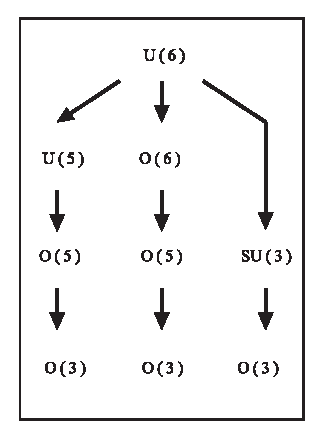
\includegraphics[scale=.65]{figure}
%
% If not, use
%\picplace{5cm}{2cm} % Give the correct figure height and width in cm
%
\caption{If the width of the figure is less than 7.8 cm use the \texttt{sidecapion} command to flush the caption on the left side of the page. If the figure is positioned at the top of the page, align the sidecaption with the top of the figure -- to achieve this you simply need to use the optional argument \texttt{[t]} with the \texttt{sidecaption} command}
\label{fig:1}       % Give a unique label
\end{figure}


\paragraph{Paragraph Heading} %
Instead of simply listing headings of different levels we recommend to let every heading be followed by at least a short passage of text. Furtheron please use the \LaTeX\ automatism for all your cross-references and citations as has already been described in Sect.~\ref{sec:2}.

Please note that the first line of text that follows a heading is not indented, whereas the first lines of all subsequent paragraphs are.

For typesetting numbered lists we recommend to use the \verb|enumerate| environment -- it will automatically render Springer's preferred layout.

\begin{enumerate}
\item{Livelihood and survival mobility are oftentimes coutcomes of uneven socioeconomic development.}
\begin{enumerate}
\item{Livelihood and survival mobility are oftentimes coutcomes of uneven socioeconomic development.}
\item{Livelihood and survival mobility are oftentimes coutcomes of uneven socioeconomic development.}
\end{enumerate}
\item{Livelihood and survival mobility are oftentimes coutcomes of uneven socioeconomic development.}
\end{enumerate}


\subparagraph{Subparagraph Heading} In order to avoid simply listing headings of different levels we recommend to let every heading be followed by at least a short passage of text. Use the \LaTeX\ automatism for all your cross-references and citations as has already been described in Sect.~\ref{sec:2}, see also Fig.~\ref{fig:2}.

Please note that the first line of text that follows a heading is not indented, whereas the first lines of all subsequent paragraphs are.

For unnumbered list we recommend to use the \verb|itemize| environment -- it will automatically render Springer's preferred layout.

\begin{itemize}
\item{Livelihood and survival mobility are oftentimes coutcomes of uneven socioeconomic development, cf. Table~\ref{tab:1}.}
\begin{itemize}
\item{Livelihood and survival mobility are oftentimes coutcomes of uneven socioeconomic development.}
\item{Livelihood and survival mobility are oftentimes coutcomes of uneven socioeconomic development.}
\end{itemize}
\item{Livelihood and survival mobility are oftentimes coutcomes of uneven socioeconomic development.}
\end{itemize}

\begin{figure}[t]
\sidecaption[t]
% Use the relevant command for your figure-insertion program
% to insert the figure file.
% For example, with the option graphics use
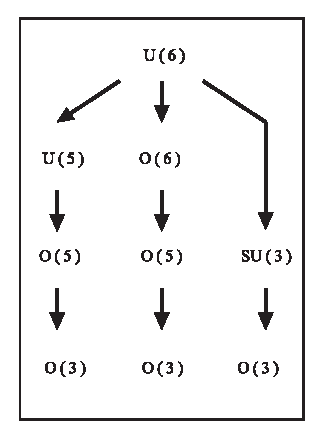
\includegraphics[scale=.65]{figure}
%
% If not, use
%\picplace{5cm}{2cm} % Give the correct figure height and width in cm
%
\caption{Please write your figure caption here}
\label{fig:2}       % Give a unique label
\end{figure}

\runinhead{Run-in Heading Boldface Version} Use the \LaTeX\ automatism for all your cross-references and citations as has already been described in Sect.~\ref{sec:2}.

\subruninhead{Run-in Heading Italic Version} Use the \LaTeX\ automatism for all your cross-refer\-ences and citations as has already been described in Sect.~\ref{sec:2}\index{paragraph}.
% Use the \index{} command to code your index words
%
% For tables use
%
\begin{table}
\caption{Please write your table caption here}
\label{tab:1}       % Give a unique label
%
% For LaTeX tables use
%
\begin{tabular}{p{2cm}p{2.4cm}p{2cm}p{4.9cm}}
\hline\noalign{\smallskip}
Classes & Subclass & Length & Action Mechanism  \\
\noalign{\smallskip}\svhline\noalign{\smallskip}
Translation & mRNA$^a$  & 22 (19--25) & Translation repression, mRNA cleavage\\
Translation & mRNA cleavage & 21 & mRNA cleavage\\
Translation & mRNA  & 21--22 & mRNA cleavage\\
Translation & mRNA  & 24--26 & Histone and DNA Modification\\
\noalign{\smallskip}\hline\noalign{\smallskip}
\end{tabular}
$^a$ Table foot note (with superscript)
\end{table}
%
%\section{Section Heading}
%\label{sec:3}
% Always give a unique label
% and use \ref{<label>} for cross-references
% and \cite{<label>} for bibliographic references
% use \sectionmark{}
% to alter or adjust the section heading in the running head
Instead of simply listing headings of different levels we recommend to let every heading be followed by at least a short passage of text. Furtheron please use the \LaTeX\ automatism for all your cross-references and citations as has already been described in Sect.~\ref{sec:2}.

Please note that the first line of text that follows a heading is not indented, whereas the first lines of all subsequent paragraphs are.

If you want to list definitions or the like we recommend to use the Springer-enhanced \verb|description| environment -- it will automatically render Springer's preferred layout.

\begin{description}[Type 1]
\item[Type 1]{That addresses central themes pertainng to migration, health, and disease. In Sect.~\ref{sec:1}, Wilson discusses the role of human migration in infectious disease distributions and patterns.}
\item[Type 2]{That addresses central themes pertainng to migration, health, and disease. In Sect.~\ref{subsec:2}, Wilson discusses the role of human migration in infectious disease distributions and patterns.}
\end{description}

\subsection{Subsection Heading} %
In order to avoid simply listing headings of different levels we recommend to let every heading be followed by at least a short passage of text. Use the \LaTeX\ automatism for all your cross-references and citations citations as has already been described in Sect.~\ref{sec:2}.

Please note that the first line of text that follows a heading is not indented, whereas the first lines of all subsequent paragraphs are.

\begin{svgraybox}
If you want to emphasize complete paragraphs of texts we recommend to use the newly defined Springer class option \verb|graybox| and the newly defined environment \verb|svgraybox|. This will produce a 15 percent screened box 'behind' your text.

If you want to emphasize complete paragraphs of texts we recommend to use the newly defined Springer class option and environment \verb|svgraybox|. This will produce a 15 percent screened box 'behind' your text.
\end{svgraybox}


\subsubsection{Subsubsection Heading}
Instead of simply listing headings of different levels we recommend to let every heading be followed by at least a short passage of text. Furtheron please use the \LaTeX\ automatism for all your cross-references and citations as has already been described in Sect.~\ref{sec:2}.

Please note that the first line of text that follows a heading is not indented, whereas the first lines of all subsequent paragraphs are.

\begin{theorem}
Theorem text goes here.
\end{theorem}
%
% or
%
\begin{definition}
Definition text goes here.
\end{definition}

\begin{proof}
%\smartqed
Proof text goes here.
\qed
\end{proof}

\paragraph{Paragraph Heading} %
Instead of simply listing headings of different levels we recommend to let every heading be followed by at least a short passage of text. Furtheron please use the \LaTeX\ automatism for all your cross-references and citations as has already been described in Sect.~\ref{sec:2}.

Note that the first line of text that follows a heading is not indented, whereas the first lines of all subsequent paragraphs are.
%
% For built-in environments use
%
\begin{theorem}
Theorem text goes here.
\end{theorem}
%
\begin{definition}
Definition text goes here.
\end{definition}
%
\begin{proof}
\smartqed
Proof text goes here.
\qed
\end{proof}
%
\begin{acknowledgement}
If you want to include acknowledgments of assistance and the like at the end of an individual chapter please use the \verb|acknowledgement| environment -- it will automatically render Springer's preferred layout.
\end{acknowledgement}
%
\section*{Appendix}
\addcontentsline{toc}{section}{Appendix}
%
When placed at the end of a chapter or contribution (as opposed to at the end of the book), the numbering of tables, figures, and equations in the appendix section continues on from that in the main text. Hence please \textit{do not} use the \verb|appendix| command when writing an appendix at the end of your chapter or contribution. If there is only one the appendix is designated ``Appendix'', or ``Appendix 1'', or ``Appendix 2'', etc. if there is more than one.

\begin{equation}
a \times b = c
\end{equation}
% Problems or Exercises should be sorted chapterwise
%\section*{Problems}
%\addcontentsline{toc}{section}{Problems}
%
% Use the following environment.
% Don't forget to label each problem;
%% the label is needed for the solutions' environment
%\begin{prob}
%\label{prob1}
%A given problem or Excercise is described here. The
%problem is described here. The problem is described here.
%\end{prob}
%
%\begin{prob}
%\label{prob2}
%\textbf{Problem Heading}\\
%(a) The first part of the problem is described here.\\
%(b) The second part of the problem is described here.
%\end{prob}

%%%%%%%%%%%%%%%%%%%%%%%%% referenc.tex %%%%%%%%%%%%%%%%%%%%%%%%%%%%%%
% sample references
% %
% Use this file as a template for your own input.
%
%%%%%%%%%%%%%%%%%%%%%%%% Springer-Verlag %%%%%%%%%%%%%%%%%%%%%%%%%%
%
% BibTeX users please use
% \bibliographystyle{}
% \bibliography{}
%
\biblstarthook{In view of the parallel print and (chapter-wise) online publication of your book at \url{www.springerlink.com} it has been decided that -- as a genreral rule --  references should be sorted chapter-wise and placed at the end of the individual chapters. However, upon agreement with your contact at Springer you may list your references in a single seperate chapter at the end of your book. Deactivate the class option \texttt{sectrefs} and the \texttt{thebibliography} environment will be put out as a chapter of its own.\\\indent
References may be \textit{cited} in the text either by number (preferred) or by author/year.\footnote{Make sure that all references from the list are cited in the text. Those not cited should be moved to a separate \textit{Further Reading} section or chapter.} The reference list should ideally be \textit{sorted} in alphabetical order -- even if reference numbers are used for the their citation in the text. If there are several works by the same author, the following order should be used: 
\begin{enumerate}
\item all works by the author alone, ordered chronologically by year of publication
\item all works by the author with a coauthor, ordered alphabetically by coauthor
\item all works by the author with several coauthors, ordered chronologically by year of publication.
\end{enumerate}
The \textit{styling} of references\footnote{Always use the standard abbreviation of a journal's name according to the ISSN \textit{List of Title Word Abbreviations}, see \url{http://www.issn.org/en/node/344}} depends on the subject of your book:
\begin{itemize}
\item The \textit{two} recommended styles for references in books on \textit{mathematical, physical, statistical and computer sciences} are depicted in ~\cite{science-contrib, science-online, science-mono, science-journal, science-DOI} and ~\cite{phys-online, phys-mono, phys-journal, phys-DOI, phys-contrib}.
\item Examples of the most commonly used reference style in books on \textit{Psychology, Social Sciences} are~\cite{psysoc-mono, psysoc-online,psysoc-journal, psysoc-contrib, psysoc-DOI}.
\item Examples for references in books on \textit{Humanities, Linguistics, Philosophy} are~\cite{humlinphil-journal, humlinphil-contrib, humlinphil-mono, humlinphil-online, humlinphil-DOI}.
\item Examples of the basic Springer style used in publications on a wide range of subjects such as \textit{Computer Science, Economics, Engineering, Geosciences, Life Sciences, Medicine, Biomedicine} are ~\cite{basic-contrib, basic-online, basic-journal, basic-DOI, basic-mono}. 
\end{itemize}
}

\begin{thebibliography}{99.}%
% and use \bibitem to create references.
%
% Use the following syntax and markup for your references if 
% the subject of your book is from the field 
% "Mathematics, Physics, Statistics, Computer Science"
%
% Contribution 
\bibitem{science-contrib} Broy, M.: Software engineering --- from auxiliary to key technologies. In: Broy, M., Dener, E. (eds.) Software Pioneers, pp. 10-13. Springer, Heidelberg (2002)
%
% Online Document
\bibitem{science-online} Dod, J.: Effective substances. In: The Dictionary of Substances and Their Effects. Royal Society of Chemistry (1999) Available via DIALOG. \\
\url{http://www.rsc.org/dose/title of subordinate document. Cited 15 Jan 1999}
%
% Monograph
\bibitem{science-mono} Geddes, K.O., Czapor, S.R., Labahn, G.: Algorithms for Computer Algebra. Kluwer, Boston (1992) 
%
% Journal article
\bibitem{science-journal} Hamburger, C.: Quasimonotonicity, regularity and duality for nonlinear systems of partial differential equations. Ann. Mat. Pura. Appl. \textbf{169}, 321--354 (1995)
%
% Journal article by DOI
\bibitem{science-DOI} Slifka, M.K., Whitton, J.L.: Clinical implications of dysregulated cytokine production. J. Mol. Med. (2000) doi: 10.1007/s001090000086 
%
\bigskip

% Use the following (APS) syntax and markup for your references if 
% the subject of your book is from the field 
% "Mathematics, Physics, Statistics, Computer Science"
%
% Online Document
\bibitem{phys-online} J. Dod, in \textit{The Dictionary of Substances and Their Effects}, Royal Society of Chemistry. (Available via DIALOG, 1999), 
\url{http://www.rsc.org/dose/title of subordinate document. Cited 15 Jan 1999}
%
% Monograph
\bibitem{phys-mono} H. Ibach, H. L\"uth, \textit{Solid-State Physics}, 2nd edn. (Springer, New York, 1996), pp. 45-56 
%
% Journal article
\bibitem{phys-journal} S. Preuss, A. Demchuk Jr., M. Stuke, Appl. Phys. A \textbf{61}
%
% Journal article by DOI
\bibitem{phys-DOI} M.K. Slifka, J.L. Whitton, J. Mol. Med., doi: 10.1007/s001090000086
%
% Contribution 
\bibitem{phys-contrib} S.E. Smith, in \textit{Neuromuscular Junction}, ed. by E. Zaimis. Handbook of Experimental Pharmacology, vol 42 (Springer, Heidelberg, 1976), p. 593
%
\bigskip
%
% Use the following syntax and markup for your references if 
% the subject of your book is from the field 
% "Psychology, Social Sciences"
%
%
% Monograph
\bibitem{psysoc-mono} Calfee, R.~C., \& Valencia, R.~R. (1991). \textit{APA guide to preparing manuscripts for journal publication.} Washington, DC: American Psychological Association.
%
% Online Document
\bibitem{psysoc-online} Dod, J. (1999). Effective substances. In: The dictionary of substances and their effects. Royal Society of Chemistry. Available via DIALOG. \\
\url{http://www.rsc.org/dose/Effective substances.} Cited 15 Jan 1999.
%
% Journal article
\bibitem{psysoc-journal} Harris, M., Karper, E., Stacks, G., Hoffman, D., DeNiro, R., Cruz, P., et al. (2001). Writing labs and the Hollywood connection. \textit{J Film} Writing, 44(3), 213--245.
%
% Contribution 
\bibitem{psysoc-contrib} O'Neil, J.~M., \& Egan, J. (1992). Men's and women's gender role journeys: Metaphor for healing, transition, and transformation. In B.~R. Wainrig (Ed.), \textit{Gender issues across the life cycle} (pp. 107--123). New York: Springer.
%
% Journal article by DOI
\bibitem{psysoc-DOI}Kreger, M., Brindis, C.D., Manuel, D.M., Sassoubre, L. (2007). Lessons learned in systems change initiatives: benchmarks and indicators. \textit{American Journal of Community Psychology}, doi: 10.1007/s10464-007-9108-14.
%
%
% Use the following syntax and markup for your references if 
% the subject of your book is from the field 
% "Humanities, Linguistics, Philosophy"
%
\bigskip
%
% Journal article
\bibitem{humlinphil-journal} Alber John, Daniel C. O'Connell, and Sabine Kowal. 2002. Personal perspective in TV interviews. \textit{Pragmatics} 12:257--271
%
% Contribution 
\bibitem{humlinphil-contrib} Cameron, Deborah. 1997. Theoretical debates in feminist linguistics: Questions of sex and gender. In \textit{Gender and discourse}, ed. Ruth Wodak, 99--119. London: Sage Publications.
%
% Monograph
\bibitem{humlinphil-mono} Cameron, Deborah. 1985. \textit{Feminism and linguistic theory.} New York: St. Martin's Press.
%
% Online Document
\bibitem{humlinphil-online} Dod, Jake. 1999. Effective substances. In: The dictionary of substances and their effects. Royal Society of Chemistry. Available via DIALOG. \\
http://www.rsc.org/dose/title of subordinate document. Cited 15 Jan 1999
%
% Journal article by DOI
\bibitem{humlinphil-DOI} Suleiman, Camelia, Daniel C. O�Connell, and Sabine Kowal. 2002. `If you and I, if we, in this later day, lose that sacred fire...�': Perspective in political interviews. \textit{Journal of Psycholinguistic Research}. doi: 10.1023/A:1015592129296.
%
%
%
\bigskip
%
%
% Use the following syntax and markup for your references if 
% the subject of your book is from the field 
% "Computer Science, Economics, Engineering, Geosciences, Life Sciences"
%
%
% Contribution 
\bibitem{basic-contrib} Brown B, Aaron M (2001) The politics of nature. In: Smith J (ed) The rise of modern genomics, 3rd edn. Wiley, New York 
%
% Online Document
\bibitem{basic-online} Dod J (1999) Effective Substances. In: The dictionary of substances and their effects. Royal Society of Chemistry. Available via DIALOG. \\
\url{http://www.rsc.org/dose/title of subordinate document. Cited 15 Jan 1999}
%
% Journal article by DOI
\bibitem{basic-DOI} Slifka MK, Whitton JL (2000) Clinical implications of dysregulated cytokine production. J Mol Med, doi: 10.1007/s001090000086
%
% Journal article
\bibitem{basic-journal} Smith J, Jones M Jr, Houghton L et al (1999) Future of health insurance. N Engl J Med 965:325--329
%
% Monograph
\bibitem{basic-mono} South J, Blass B (2001) The future of modern genomics. Blackwell, London 
%
\end{thebibliography}

% BibTeX users please use
\bibliographystyle{spbasic} %plain, harvard, apalike, chicago, astron, authordate, natbib.
\bibliography{bibliography}

